%! TEX root = ../main.tex
\documentclass[../main]{subfiles}

\begin{document}
\chapter{部誌テンプレートの機能紹介} % タイトル
\rightline{4年 森山 陽介} % 学年と名前(ハンドルネームでも可)
\section{ディレクトリ構造}
\begin{verbatim}
  + .devcontainer
  |- devcontainer.json
  |- setup.sh
  + .github
  + .vscode
  |- extensions.json
  |- latex.code-snippets
  |- setting.json
  + bin
  + classes
  :
  |- supernova.cls
  + cover
  + figures
  + font
  + out
  + sections
  .gitignore
  .latexmkrc
  :
  preamble.tex
  :
  super_nova_20yy.tex

\end{verbatim}
\verb|.devcontainer|は\LaTeX 環境を構築するDevcontainerの設定ファイルが格納されている。

\verb|.vscode|には、\LaTeX を書く上で便利なスニペット(ショートカット)や設定が格納されている。

基本的に、\verb|super_nova_20yy.tex|をmainとして、その中身の内容はsectionsディレクトリに章ごと(人ごと)にtexファイルを分割して読み込む形になっている。sectionsディレクトリに、投稿された記事ごとのサブディレクトリを作って、その中に原稿ファイルと画像ファイルを一緒に保存する(画像ファイルはまた別にfigureディレクトリに保管するのもアリ)
\section{部誌の構造}
以下が、部誌の根幹部分になる\verb|super_nova_20yy.tex|のソースコードである。
\lstinputlisting{main.tex}
オリジナルのクラスファイル\verb|classes/supernova.cls|を読み込んで、原稿は\verb|\subfile{hogehoge}|の形式で読み込んでいる。この\verb|hogehoge|の部分には、読み込みたいtexファイルのパスを指定してあげれば良い。
\subsection{原稿記事の書式}
\verb|\subfile{hogehoge}|で読み込む記事のテンプレートがこちら
\begin{lstlisting}
  %! TEX root = ../supernova_20yy.tex
  \documentclass[../super_nova_20yy]{subfiles}
  
  \begin{document}
  \chapter{タイトル} % タイトル
  \rightline{5年 電通 太郎} % 学年と名前(ハンドルネームでも可)
  
  
  \end{document}
\end{lstlisting}
\verb|\documentclass[../super_nova_20yy]{subfiles}|とすることで、親ファイルのクラス設定が引き継がれてサブファイル単体でもコンパイルすることができる。\footnote{何故かできるやつとできずにエラー吐かれるのがあるけど、よくわかってない}

そして、部誌編集担当の主な仕事は投稿された原稿をこのサブファイルの書式に直していくことになる。といっても、プリアンブルに追加パッケージがないかだけ確認して(あったら親ファイルのプリアンブルに追記)、サブファイルの書式に書き換えるだけ。

ひとつ、注意したいのが図の読み込みなどに関してで、サブファイルからの\verb|\includegraphics|などでは、
\begin{lstlisting}
  \begin{figure}[H]
    \centering
    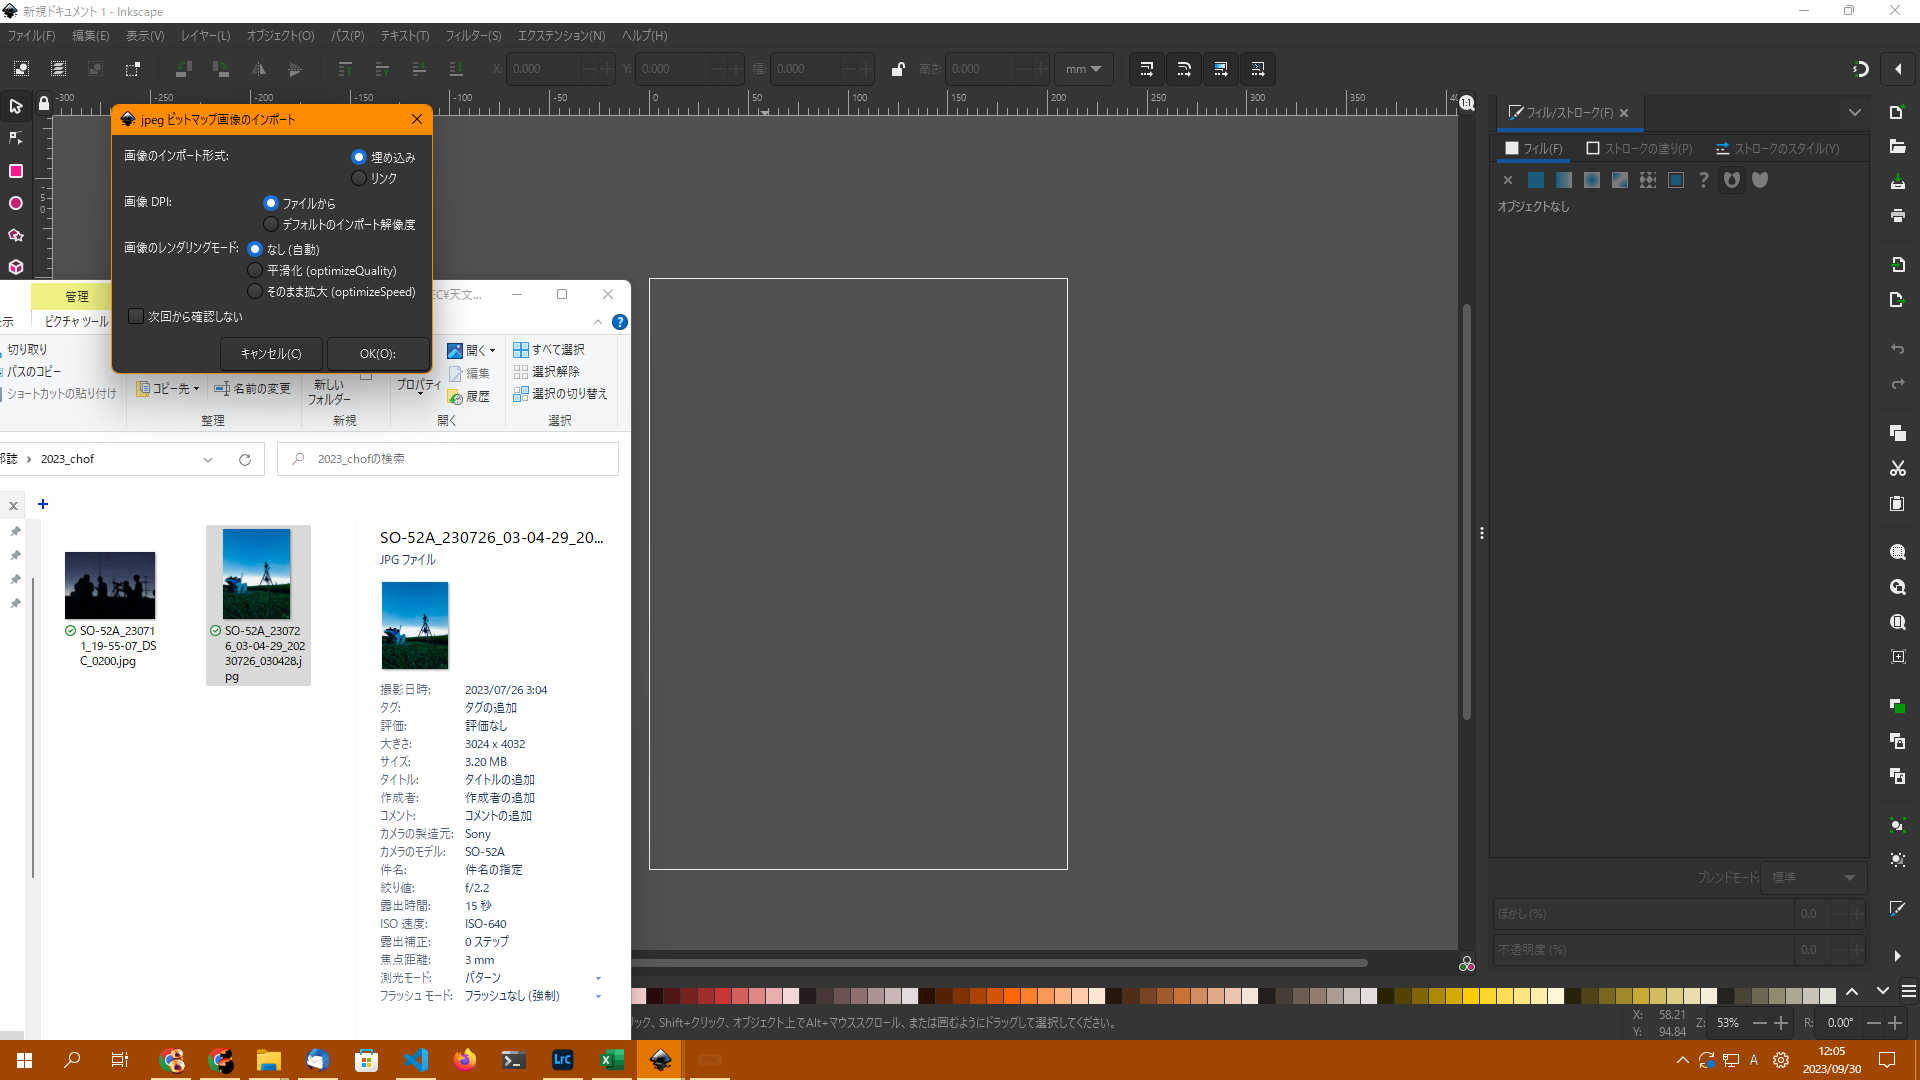
\includegraphics[width=.5\textwidth]{figures/ss265.png}
    \caption{表紙にしたい画像をドラッグ・アンド・ドロップ}
    \label{fig:ss265}
  \end{figure}
\end{lstlisting}
と言ったように、サブファイルからみた相対パスではなく、親ファイル(ルート)からみた相対パスを書き込まなければならないことに注意

\section{部誌の書式設定}
詳しくは、\verb|supernova.cls|を参照してみてほしいが、
\begin{lstlisting}
\NewPageStyle{astrobook}{ % 生TeX原稿での柱とノンブルの設定
  yoko,
  odd_running_head=_section,
  even_running_head=_chapter,
  running_head_position=top-fore-edge,
  nombre_position=bottom-fore-edge
}
\pagestyle{astrobook} % 上の設定を適用
\end{lstlisting}
では、ページ上部のページ説明欄(柱)とページ下部のページ数表記(ノンブル)の設定を行っている。texファイルで書かれた原稿には、これらの設定が反映されるが、PDFで入稿されたページを普通に\verb|\includepdf|などで読み込むとこの設定は反映されず、柱は良いとしてもページ数が飛んでしまうなどして統一感を損ねる。そこで、PDF原稿の読み込みには
\begin{lstlisting}
\newcommand{\article}[4][-]{ % PDF原稿の読込みマクロの設定
  \markboth{#2}{#3}
  \phantomsection % hyperrefおよびPDFのブックマークに表示させる
  \addcontentsline{toc}{chapter}{#2}% 個々のタイトルなどは目次ではchapter扱い
  \includepdf[pages=#1, noautoscale=true, fitpaper, pagecommand={}]{#4}
}
\end{lstlisting}
で定義したコマンドによって、\verb|\article{題名}{著者}{ファイル名}|のようにして読み込む。このとき、\verb|\article[1]{題名}{著者}{ファイル名}|というようにすれば、読み込みたいPDF原稿の1ページ目だけが読み込まれることになる。\verb|[1-3]|というようにすれば1ページ目から3ページ目まで読み込むことになる。詳しくは、\verb|\includepdf|のpagesオプションについて参照してほしい。
\subsection{スニペットと図表参照の簡便化}
クラスファイルの末尾に
\begin{lstlisting}
  % 図表番号を参照するときに図\ref{hoge}とかしなくて言いようにするマクロ
  \newcommand{\figref}[1]{図\ref{fig:#1}}
  \newcommand{\tabref}[1]{表\ref{tab:#1}}
  %\newcommand{\eqref}[1]{式(\ref{eq:#1})}
  \renewcommand{\eqref}[1]{式(\ref{eq:#1})}
\end{lstlisting}
を追加している。これによって、図表の参照が楽になる。

ただし、図表の\verb|\label|を宣言するときに\verb|\label{fig:hogehoge}|といった具合に、図なら[fig:], 表なら[tab:], 数式なら[eq:]を書いておく必要がある。\footnote{え、めんどいって?いや、これがあるおかげで助かるときもあるんだよ}
そして、めんどくさいのが、図や表を書くときのコマンド群を羅列することだが、スニペットを設定してあるので、"figure"と打ってtabを押すなどして変換候補を確定すれば
\begin{figure}
  \centering
  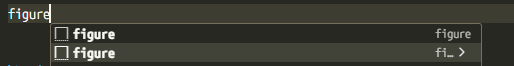
\includegraphics[width=.5\textwidth]{figures/ss275.png}
  \caption{figureと入力して変換候補を確定}
  \label{fig:snippets}
\end{figure}
\begin{lstlisting}
\begin{figure}
  \centering
  \includegraphics[width=.5\textwidth]{}
  \caption{}
  \label{fig:}
\end{figure}
\end{lstlisting}
が出てくる。同じように"table"と打てば
\begin{lstlisting}
\begin{table}
  \centering
  \caption{}
  \label{tab:}
  \begin{tabular}{}\hline
    
  \end{tabular}
\end{table}
\end{lstlisting}
が出てくるし、"doublefigure"や"doubletable"と打てば横に並んだ2つの図や表のテンプレートも出てくる。呼び出す名前は\verb|.vscode/latex.code-snippets|のファイル内の"prefix"に該当する部分の名前を入力すれば良い。

\section{さいごに}
ここまでが大体の流れになる。これを基に使いやすいように作り替えてくれて構わないし、これを基にしてくれなくても構わない。他にもいろんな機能をつけたり、統一感を出すために泥臭い工夫した記憶もあるけれど、書ききれないので、過去のファイルをドライブから漁って参考にしてみてほしい。良い部誌ができることを期待している。

\end{document}
